As the mobile workload dataset, we use an extended version of the PocketData~\cite{kennedy2015pocket} dataset which provides handset-based data directly collected from smartphones for multiple users.
It includes
%one month's
20 day's
trace of SQLite activity of
%11
\note{60}
PhoneLab~\cite{phonelab} smartphones running the Android smartphone platform.

This dataset consists of various information about the usage patterns across a wide variety of apps, and ot is a best-effort anonymized dataset.
Most of the private information is irreversibly concealed but there are still some constants in the queries.

The older version of the dataset that includes a month's trace of SQLite activity of 11 users is available online~\cite{kennedy2015pocket}.
\note{However, the data that we used in this paper is only available by request, and the researchers has to follow the IRB requirements of their institute to be able to use, and publish using this data.}

%Each line in the log has:

%\begin{itemize}
%  \item Device ID: Unique identifier for each device
%  \item UNIX timestamp: Milliseconds since 1970
%  \item Ordering: Timestamp and request order
%  \item Date and time: Human readable timestamp
%  \item Process ID: Standard UNIX process ID
%  \item Thread ID: Standard UNIX thread ID
%  \item Log level: Verbose (V), Debug (D), Info (I), Warning (W), Error (E) 
%  \item Tag: Source of log information, ``SQLite-Query-PhoneLab''
%  \item JSON object that holds various information about the event that is logged
%\end{itemize}

%information.

%Note that the app ID is not included in the log, because different apps can have the same process and thread IDs in different times.
%Our strategy to get the log lines for our app of interest is to search for the app name in JSON object parsing from the beginning of the file.
%When we first encounter the app of interest, we use process and thread IDs to identify the events related to that app until we encounter a different app name in the JSON object.

%Hence, we implement all the functions of the system with Java for it to be repackaged, and be able to be imported into mobile phones as well as servers.
%This may solve the privacy concerns of the users: allowing the processing to be performed on the phone instead of a company server even if it is not the ideal case due to performance and energy consumption constraints.

\subsection{Environment}

In our experiments regarding clustering, we used an Apple Macbook Pro with macOS Sierra operating system, 2.7 GHz Intel Core i5 processor, 8GB RAM, Java 1.8 SE Runtime Environment and R v3.3.2.

In our experiments regarding pattern matching, we used a Lenovo Thinkpad with Windows 10, 2.3 GHz Intel Core i5 processor, 8GB RAM, Java 1.8 SE Runtime Environment and R v3.3.1.

\subsection{Clustering}

For our experiments, we selected Facebook to be our example app. For visual purposes, we clustered the activities of only one user in Figure~\ref{fig:dendrogram}. For this specific user's case, there are 84273 rows of activities in the log. There are 8795 parsable select queries, however, there are only 59 unique queries among them. Keep in mind that PocketData dataset is an anonymized dataset where most of the constant values are replaced with ``?'', which reduces the number of distinct queries greatly. The dendrogram we created using Makiyama method and hierarchical clustering can be seen in Figure~\ref{fig:dendrogram}.

\begin{figure}[h!]
    \centering
    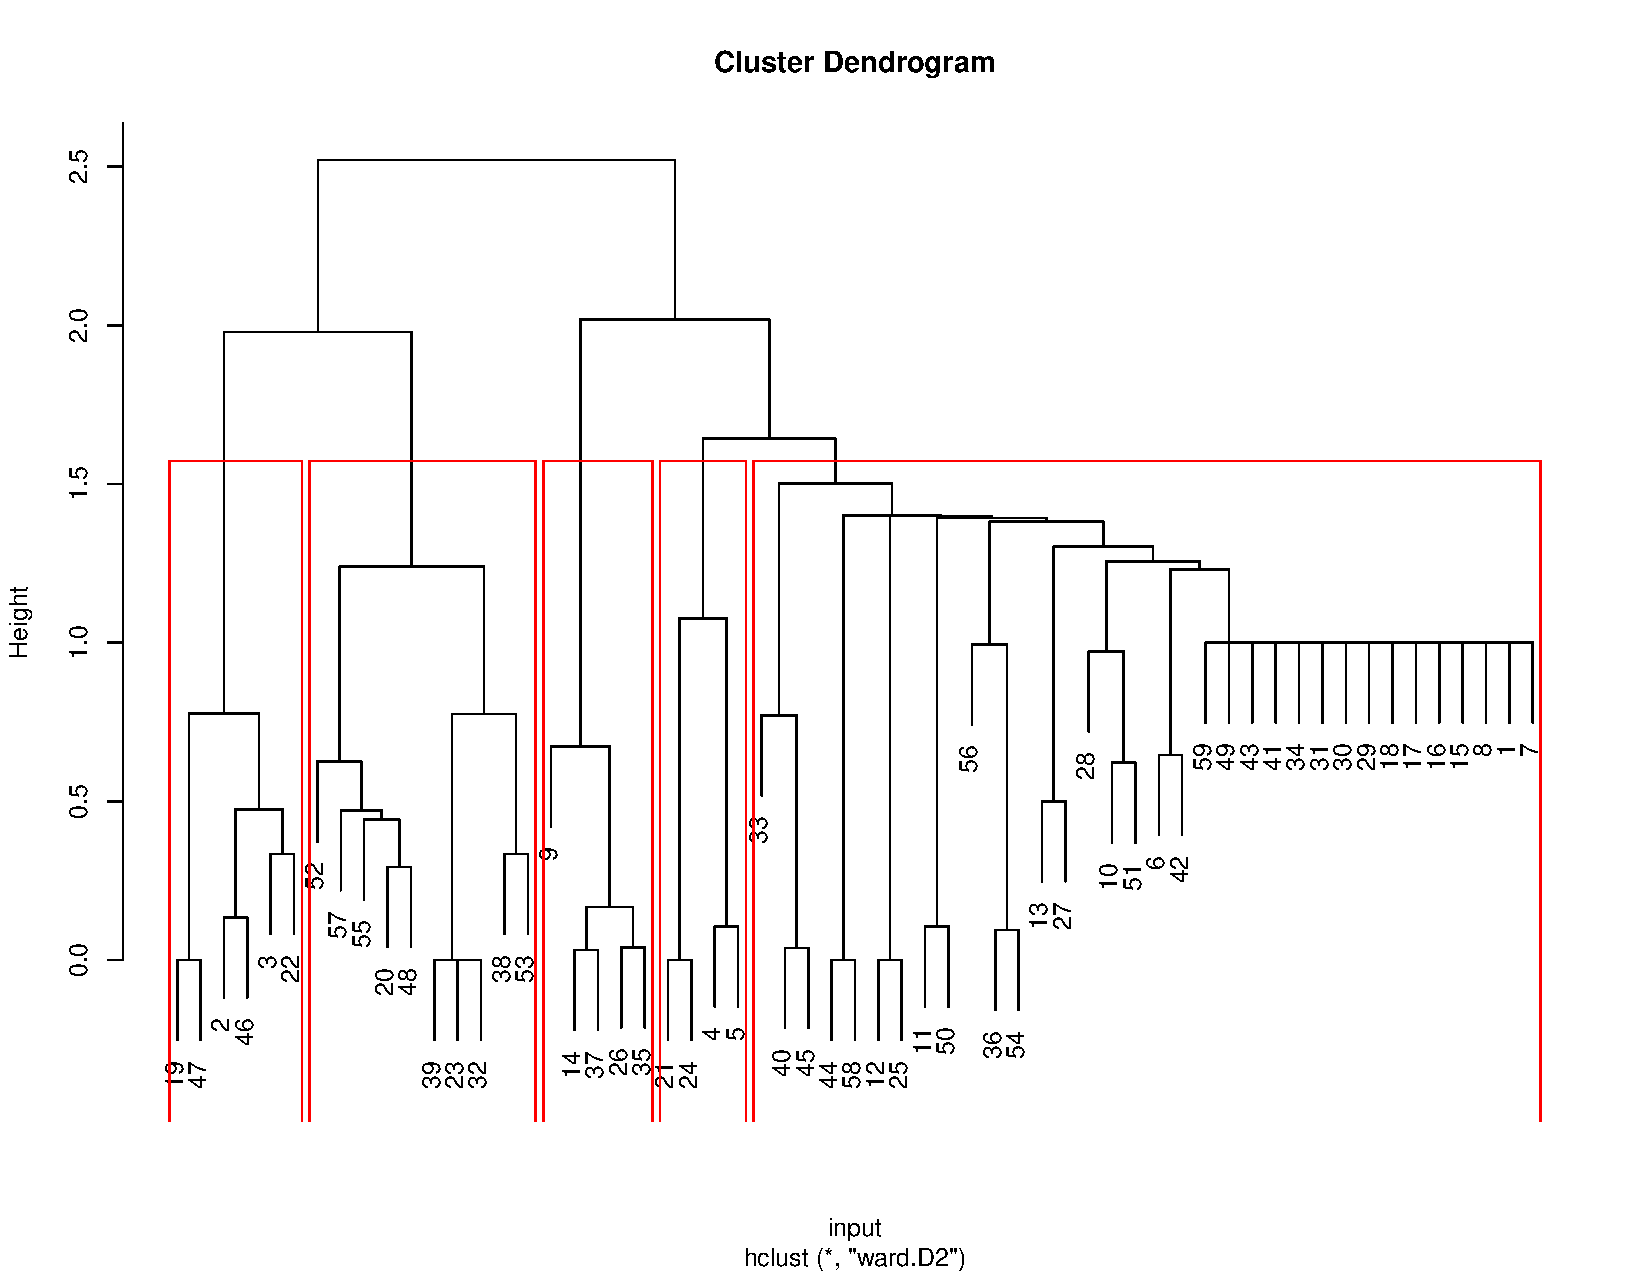
\includegraphics[width=0.5\textwidth]{graphics/User1}
    \caption{Makiyama Clustering Dendrogram of Facebook usage for a user}
    \label{fig:dendrogram}
\end{figure}

As random examples, here are some the queries that are put in the same clusters:

\begin{verbatim}
Cluster 1:
19 -> SELECT seen_state,
             updated,
             cursor,
             cache_id,
             dashing,
             icon_uri,
             photo_uri,
             profile_picture_uri,
             summary_graphql_text_with_entities, 
             short_summary_graphql_text_with_entities,
             notif_id,
             star_rating
      FROM gql_notifications
      WHERE (recipient_id=?)
      ORDER BY updated DESC LIMIT ?

3 -> SELECT cursor
     FROM gql_notifications
     WHERE (recipient_id=?)
     ORDER BY updated DESC LIMIT 1

Cluster 4:

4 -> SELECT timestamp,
            data,
            fetchreason
     FROM cache
     WHERE cachekey= ?

21 -> SELECT value, timestamp
      FROM cache
      WHERE (name='MFacewebVersion:MRootVersion')
      ORDER BY name DESC

\end{verbatim}

As seen in Figure~\ref{fig:dendrogram}, there are 5 different clusters of queries when clustered with Makiyama method. In Table~\ref{tab:clusteringresult}, we provide the tasks performed by the queries within the corresponding cluster.

\begin{table}[h!]
\centering
\caption{Makiyama lustering results}
\label{tab:clusteringresult}
\begin{tabular}{|c|c|}
\hline
Cluster & Explanation                        \\ \hline
1       & New notification check             \\ \hline
2       & Prefetch and retrieve notification \\ \hline
3       & Fill home feed                     \\ \hline
4       & Cache operations                   \\ \hline
5       & Housekeeping                       \\ \hline
\end{tabular}
\end{table}


Also, for the n-gram approach, when we choose n to be 2, we created the clustering shown in Figure~\ref{fig:ngram}.

\begin{figure}[h!]
    \centering
    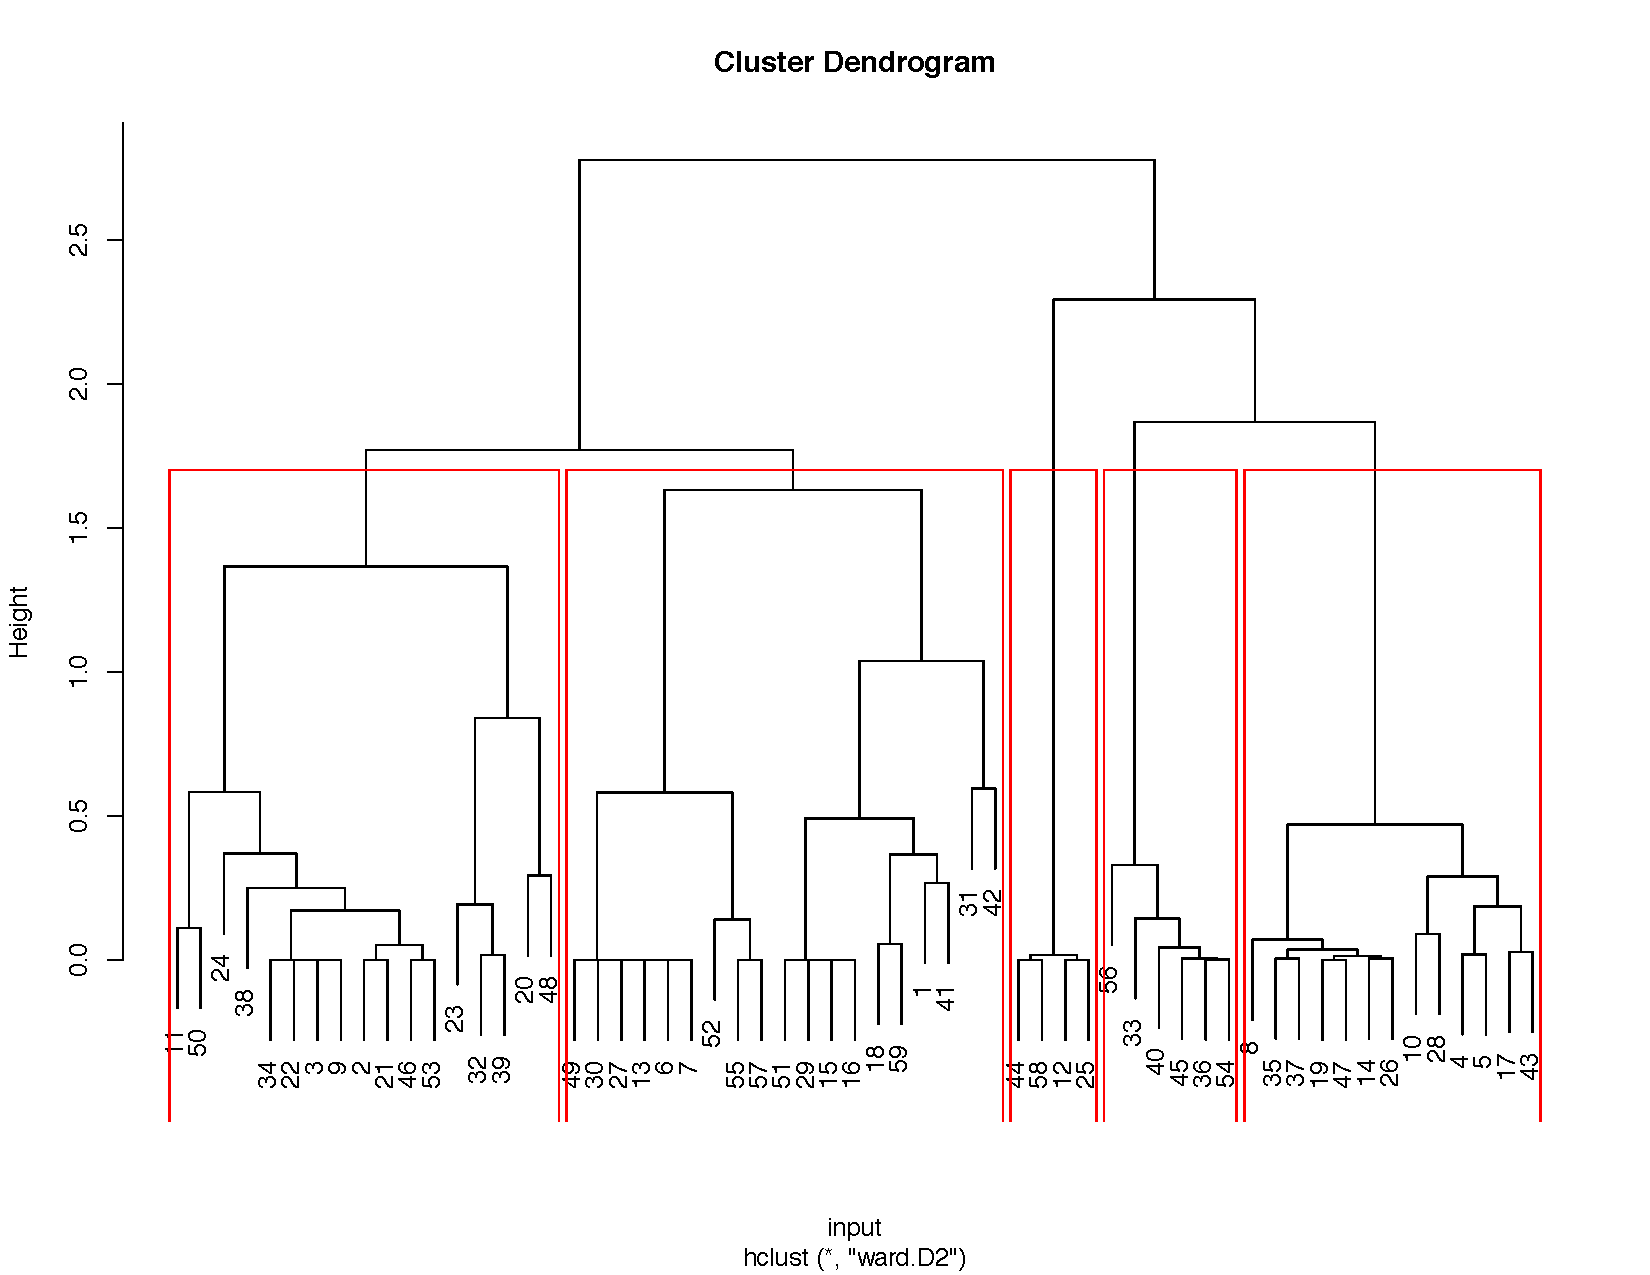
\includegraphics[width=0.5\textwidth]{graphics/Ngram}
    \caption{N-Gram Clustering Dendrogram of Facebook usage for a user}
    \label{fig:ngram}
\end{figure}

In Table~\ref{tab:clusteringresultngram}, we provide the explanations for the queries according to the clusters they got appointed with n-gram feature extraction scheme.

\begin{table}[h!]
\centering
\caption{N-Gram clustering results}
\label{tab:clusteringresultngram}
\begin{tabular}{|c|c|}
\hline
Cluster & Explanation                       \\ \hline
1       & Key-Value lookups                 \\ \hline
2       & No filter or multiple row lookups \\ \hline
3       & Lookup in a provided list         \\ \hline
4       & Complex queries                   \\ \hline
5       & Top-k row queries                 \\ \hline
\end{tabular}
\end{table}

We also created a tanglegram to show how similar clusterings these two methods created in Figure~\ref{fig:tanglegram}. As can be seen in the figure, there is little to no similarity between these clusterings which is not unexpected since the two feature extraction mechanisms completely have different strategies and targets different features.

\begin{figure*}[h!]
    \centering
    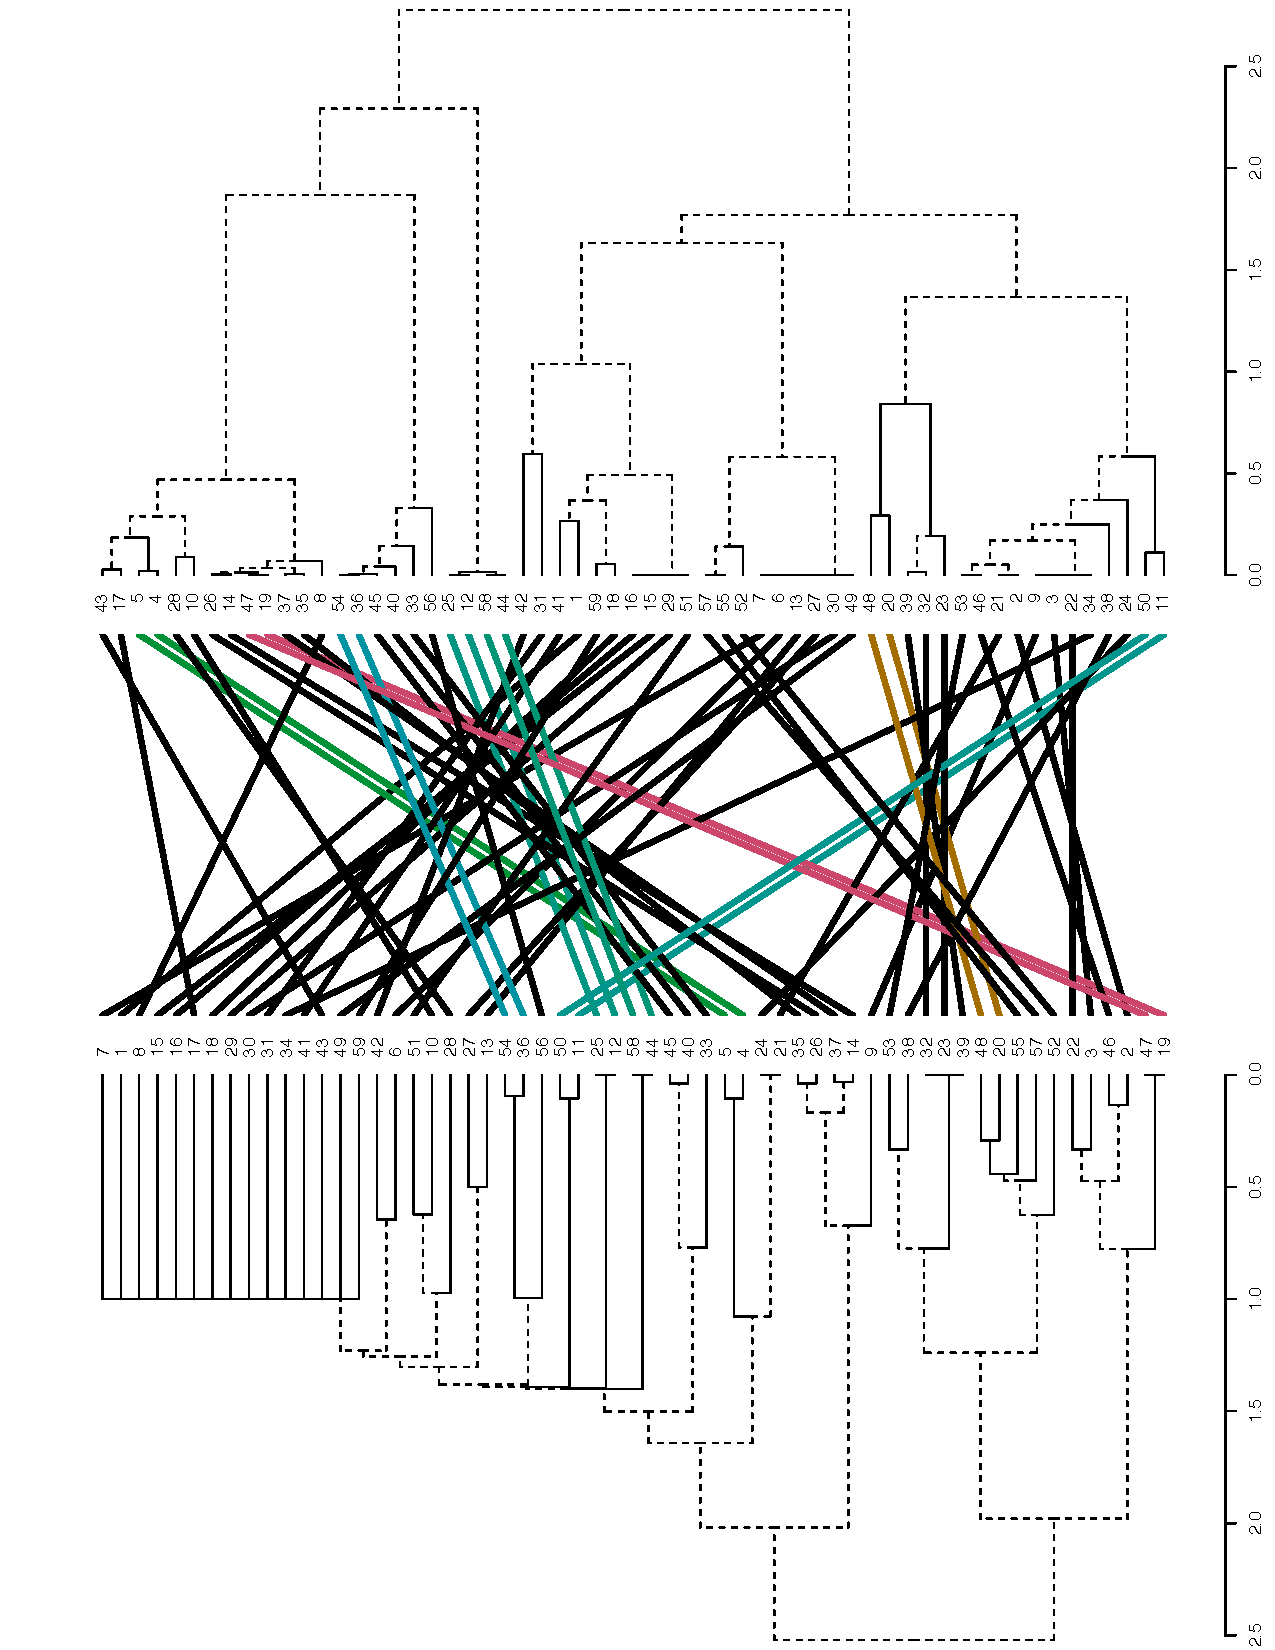
\includegraphics[width=0.9\textwidth]{graphics/tanglegram}
    \caption{Matching of n-gram clustering (on the top) and Makiyama clustering (on the bottom)}
    \label{fig:tanglegram}
\end{figure*}



\subsection{Session Identification}

The first set of experiments were directed towards coming up with an idle time tolerance. We ran our user sessions segmentation routine for query logs of 3 users for the timeline of a month. The idle time tolerances used were 10ms, 100ms, 1s, 5s, 10s, 1min, 2min and 5min. We noticed that the number of user sessions generated converged to around 10000 milliseconds of idle time tolerance as can be seen in Figure~\ref{fig:idletime}. So, we chose an idle time of 10 seconds for further experiments.

\begin{figure*}[h!]
    \centering
    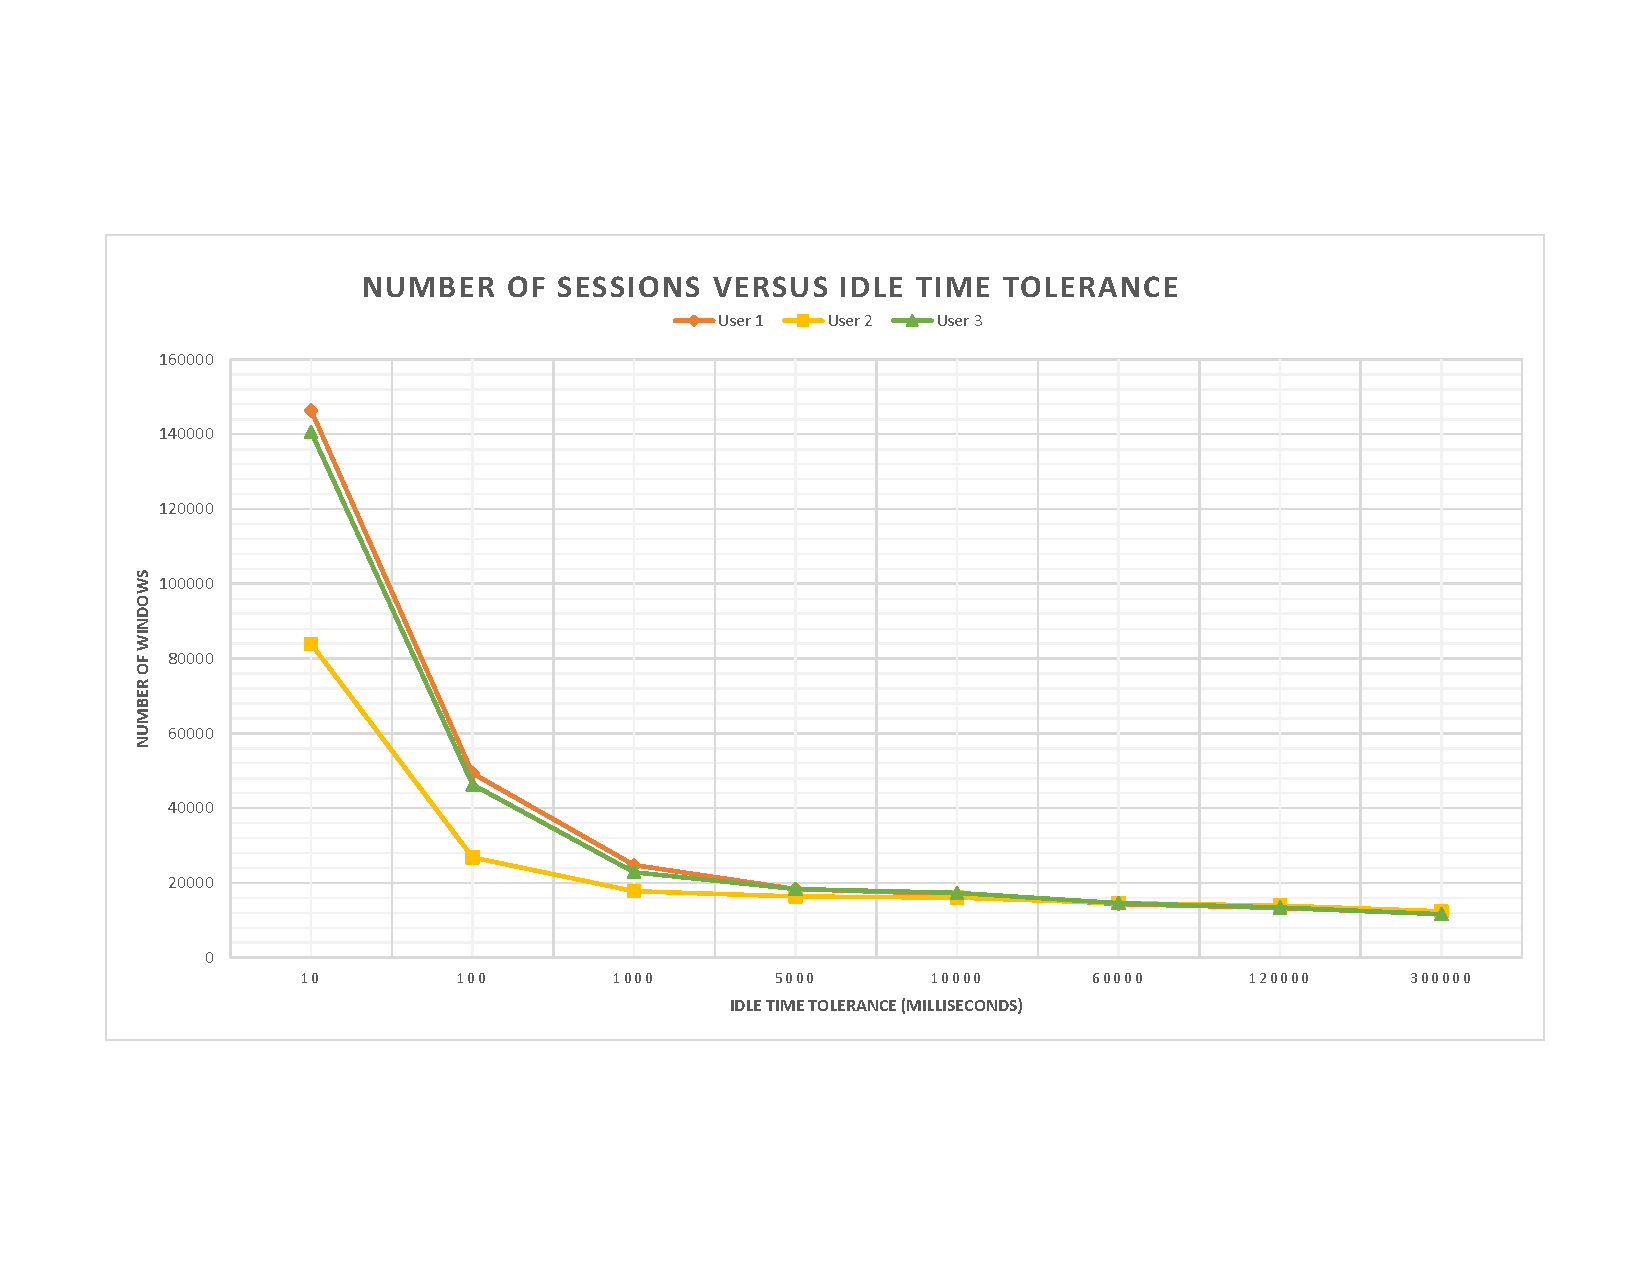
\includegraphics[width=0.9\textwidth]{graphics/IdleTimeTolerances}
    \caption{Number of user sessions generated with varying idle time tolerances}
    \label{fig:idletime}
\end{figure*}

While the idea of a low idle time tolerance might be enticing because it enables us to look into the query log at a more granular level, we decided that this approach was more suitable. When the number of user sessions became too high, neighboring sessions started to become very similar to each other. This might lead to a myopic view of the data. Also, it is reasonable to hypothesize that the general usage pattern of smartphones is in bursts. The user would pickup the smartphone for a few minutes, perform a bunch of tasks and then keep it away. During these bursts of activity, the high similarity among smaller user sessions could be because of the fact that if a user is checking the Facebook feed for 5 seconds, it is highly probably that they will keep doing that for the next many seconds. However, we are able to deal with this myopic view with larger idle time tolerances. Also, higher idle time tolerances lead to lower number of user session windows. The time complexity of similarity calculation operation is $O(n^2)$. Higher idle time tolerances fit the general usage patterns, as well as, reduce the computational complexity of calculating the average similarity vector.

\subsection{Common patterns}

Extracting meaningful patterns from user data is central to a reliable characterization of the smartphone database workload. We proposed a robust similarity measure which takes into the account the considerations and constraints that are imposed by the problem domain. We believe that our experimental results support the dependability of this approach for mobile applications. 

We applied the idle time treshold as 10 seconds over the Facebook query set for a month of usage for 11 users as we indicated in the previous section in order to determine how many sessions there are. This operation revealed that there were 15820 sessions initiated in the dataset according to the session definition. Among these 15820 sessions, 5184 of them had 90\% or higher average similarity with all other sessions and there are 25 sessions that had 25\% or less average similarity with all other sessions as show in Figure~\ref{fig:averagesimilarity}.

\begin{figure*}[h!]
    \centering
    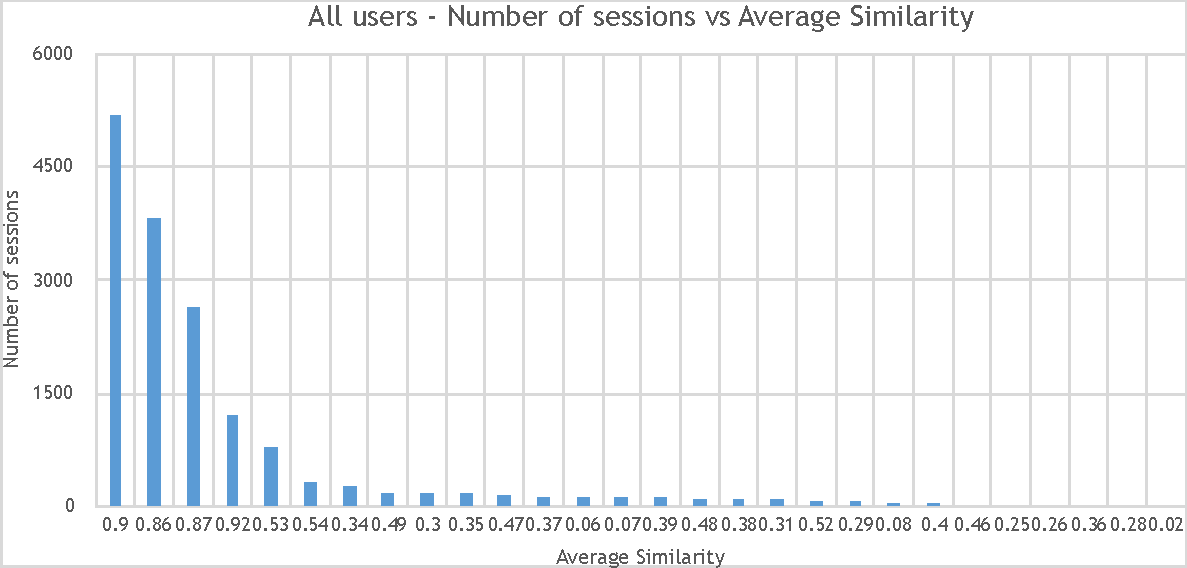
\includegraphics[width=0.9\textwidth]{graphics/allsessions}
    \caption{Number of sessions separated by their average similarity}
    \label{fig:averagesimilarity}
\end{figure*}

We believe that a random session selection among the 5184 sessions can provide us with a representative query set of the workloads for all users since 90\% average similarity means the query set represents 90\% of all the sessions in the dataset. The average, minimum and maximum session lengths are given in Table~\ref{tab:sessionlength}.

\begin{table*}[h!]
\centering
\caption{Session length}
\label{tab:sessionlength}
\begin{tabular}{ccccl}
\cline{1-4}
\multicolumn{1}{|c|}{}                                        & \multicolumn{1}{c|}{Average Session Length} & \multicolumn{1}{c|}{Minimum Session Length} & \multicolumn{1}{c|}{Maximum Session Length} &  \\ \cline{1-4}
\multicolumn{1}{|c|}{Sessions with 90\% or higher similarity} & \multicolumn{1}{c|}{3474.32 ms}                      & \multicolumn{1}{c|}{10 ms}                      & \multicolumn{1}{c|}{159320 ms}                      &  \\ \cline{1-4}
\multicolumn{1}{|c|}{Sessions with 25\% or less similarity} & \multicolumn{1}{c|}{2402.91 ms}                      & \multicolumn{1}{c|}{4 ms}                      & \multicolumn{1}{c|}{136110 ms}                      &  \\ \cline{1-4}
\multicolumn{1}{|c|}{All sessions}                            & \multicolumn{1}{c|}{5065.02 ms}                      & \multicolumn{1}{c|}{4 ms}                      & \multicolumn{1}{c|}{218959 ms}                      &  \\ \cline{1-4}
\multicolumn{1}{l}{}                                          & \multicolumn{1}{l}{}                        & \multicolumn{1}{l}{}                        & \multicolumn{1}{l}{}                        & 
\end{tabular}
\end{table*}

As for outlier detection, the 25 sessions that have 25\% or less average similarity is a very moderate number that should be inspected to understand the structure of extraordinarily different sessions.





